\section{Materialien}\label{sec:Materialien}
In den nachfolgenden Abschnitten, werden Werkzeuge und Hilfsmittel beschrieben, die für die Fertigstellung des Projekts vonnöten waren.\\ Des weiteren werden auch Komponenten vorgestellt, die während der Projektlaufzeit erstellt wurden, wie etwa die Würfel-Marker (s. Abb.~\ref{fig:marker}).

\subsection{Hardware}
Zur Ausführung der \emph{MArC}-Software sind diverse Hardware-Komponenten Voraussetzung. Diese Komponenten werden nachfolgend beschrieben und deren Kontext im System näher erläutert.
\subsubsection{Computer zur Ausführung der Unity-Simulation}\label{sec:UnityComp}\todo[inline, color=yellow] {Lukas}
Die Anwendung, welche aus Unity \cite{website:Unity} heraus erstellt wurde, benötigt einen Host-Computer, welcher sowohl mit dem HTC Vive Head-Mounted Display kompatibel, als auch leistungsstark genug sein muss, um das Rendering der Simulation mit ausreichend hoher Bildrate ausführen zu können.

Für das vorliegende Projekt wurde seitens der Technischen Hochschule Köln ein Computer zur Verfügung gestellt. Die technischen Daten des Geräts sind in Tabelle~\ref{tab:UnityCompParam} aufgeführt.

\begin{table}
	\centering
	\begin{tabular}{|l|l|}
		\hline
		\Absatzbox{}
		\textbf{CGPC6}& \textbf{Beschreibung} \\
		\hline
		Prozessor & Intel Core i7 6700 CPU \@ $2 \times 3.4$GHz \\
		\hline
		Arbeitsspeicher & $16$ GB \\
 		\hline 
		Grafikkarte & NVIDIA GeForce GTX 980\\
		\hline
		Betriebssystem & Windows 10 Education 64 bit \\
		\hline
		Schnittstellen & $2\times$ USB 3.0, $5 \times$ USB 2.0, $1 \times $ HDMI \\
		\hline
	\end{tabular}
	\caption{Auszug aus dem technischen Datenblatt des XXXX.}
	\label{tab:UnityCompParam}
\end{table}

Die Hard- und Software-Voraussetzungen für die Ausführung der Unity-Anwendung in Verbindung mit der HTC Vive, welche in Tabelle~\ref{tab:viveReq} aufgelistet sind, werden von dem verwendeten Computer übertroffen.

\begin{table}
	\centering
	\begin{tabular}{|l|l|}
		\hline
		\Absatzbox{}
		\textbf{HTC Vive}& \textbf{Systemvoraussetzungen} \\
		\hline
		Prozessor & mindestens Intel Core i5-4590 oder AMD FX 8350\\
		\hline
		Grafikkarte & mindestens NVIDIA GeForce™ GTX 1060\\
		&oder AMD Radeon™ RX 480\\
		\hline
		Arbeitsspeicher & mindestens $4\,GB$\\		
		\hline
		Videoausgang & $1\times$ HDMI 1.4-Anschluss oder DisplayPort 1.2\\
		\hline
		USB & $1\times$ USB 2.0-Anschluss\\
		\hline
		Betriebssystem & Windows 7 SP1, Windows 8.1 oder Windows 10\\
		\hline
	\end{tabular}
	\caption{HTC Vive Systemvoraussetzungen. \cite{website:HTC_Vive_Ready}}
	\label{tab:viveReq}
\end{table}

\subsubsection{Computer zur Ausführung der Tracking-Anwendung}\label{sec:TrackingComp}\todo[inline, color=green]{Vera}

Auf Grund der begrenzten Bandbreite einer USB-Karte ist es zwingend notwendig einen weiteren Rechner an das Gesamtsystem zu koppeln, welcher ausschließlich für die Ansteuerung der uEye-Kamera und die Berechnungen des Tracking-Algorithmus zuständig ist. 
An den Computer zur Ausführung der VR Umgebung sind gezwungenermaßen viele externe USB Komponenten, wie zum Beispiel die \textit{Leap Motion} und die \textit{HTC Vive}, angeschlossen. Dies führt zu einer hohen Auslastung der Bandbreite der USB-Karte und auf Grund dessen ist es nicht mehr möglich die uEye-Kamera mit der notwendigen maximalen Framerate zu betreiben. Somit wird für ein flüssiges und real-time fähiges Tracking der \textit{Acer E5-571G-795A} mit den Eigenschaften aus Tabelle \ref{tab:TrackingCompParam} verwendet.

\begin{table}
	\centering
	\begin{tabular}{|c|c|}
		\hline
		\Absatzbox{}
		\textbf{Acer E5-571G-795A}& \textbf{Beschreibung} \\
		\hline
		Prozessor & Intel Core i7-5500U CPU @ $2\times 2.4$GHz  \\
		\hline
		Arbeitsspeicher & $8.0$ GB \\
		\hline 
		Grafikkarte & NVIDIA GeForce 840M\\
		\hline
		Betriebssystem & Windows 10 Home, 64 bit \\
		\hline
		Schnittstellen & $2\times$ USB 2.0, $1\times$ USB 1.0, Netzwerkport ????\\
		\hline
	\end{tabular}
	\caption{Auszug aus dem technischen Datenblatt des \textit{Acer E5-571G-795A}.}
	\label{tab:TrackingCompParam}
\end{table}


\subsubsection{HTC Vive}\label{sec:Vive} \todo[inline, color=green]{Laura}
Bei der \textit{HTC Vive} handelt es sich um ein Head-Mounted Display, welches von \textit{HTC} in Kooperation mit \textit{Valve} \cite{website:Valve} produziert wird. Vorgestellt wurde dieses am 1. März 2015 im Vorfeld des \textit{Mobile World Congress} \cite{website:mobileworldcongress}.\\
Die Auflösung des Displays beträgt insgesamt $2160\times1200$ Pixel, was $1080\times1200$ Pixeln pro Auge enstpricht. Die Brille bietet ein Sichtfeld von bis zu $110^\circ$ bei einer Bildwiederholrate von $90\,Hz$ \cite{website:HTC_Vive}. Alle technischen Systemvoraussetzungen können in Tabelle \ref{tab:viveReq} eingesehen werden. \\
Zur Positionsbestimmung im Raum wird die Lighthousetechnologie von \textit{Valve} genutzt. Zusätzlich sind neben einem Gyrosensor auch ein Beschleunigungsmesser und ein Laser-Positionsmesser verbaut. Mittels speziellen Game-Controllern wird eine Interaktion mit virtuellen Objekten ermöglicht.

\subsubsection{IDS uEye 164LE-C}\label{sec:uEye} \todo[inline, color=green] {Vera}
Die Kamera \textit{uEye 164LE-C} wurde vom Hersteller \textit{IDS Imaging Development Systems} entwickelt. Sie hat eine Auflösung von $1280 \times 1024$ Pixel und ermöglicht Live-Video-Aufnahmen im RGB Farbmodus mit maximal $25$ fps. Der integrierte CMOS Bildsensor wird im Rolling Shutter betrieben und ermöglicht Belichtungszeiten von $37\mu$s bis $10$s. Weiterführend kann sie universell mit allen gängigen Computern oder Systemen via USB 2.0 Schnittstelle verbunden werden \cite{website:UEyeTechSpec}.\\

Die erforderliche Ansteuerung der \textit{uEye 164LE-C} erfolgt mit Hilfe der bereit gestellten \textit{IDS Software Suite}. In diese Suite ist die \textit{uEye-API} integriert, welche die Entwicklung von eigenen Programmen unter \textit{Windows} und \textit{Linux} mit den Programmiersprachen \textit{C}$++$, \textit{.NET}, \textit{C$\#$} oder \textit{C} ermöglicht \cite{website:IDSSuite}. Für das Tracking der Marker in \textit{MArC} wurde eine eigene Schnittstelle in \textit{C}$++$ erstellt, welche die Kamera im Live Modus initialisiert und steuert. 


\subsubsection{Leap Motion}\label{sec:LeapMotion} \todo[inline,color=green]{Paul}	
Bei der \textit{Leap Motion} \cite{website:LeapMotion} handelt sich um ein $7,6\times3\times1,3\,cm$ großes Gerät, welches es mit Hilfe von Sensoren möglich macht, Hand- und Fingerbewegungen zu tracken und diese als Eingabemöglichkeit zu nutzen. Die Idee dahinter ist, eine Eingabegerät im virtuellen Raum analog zu Maus zu schaffen, welches keinen direkten Kontakt bzw. keine Berührung benötigt. Hergestellt wird die \textit{Leap Motion} von der amerikanischen Firma Leap Motion Inc. Gegründet wurde die Firma am 1. November 2010. \\
Wie auf Abbildung \ref{fig:leapMotion} gezeigt, besteht das Gerät im wesentlich aus zwei integrierten weitwinkel Kameras und drei einfachen Infrarot LEDs. Die LEDs haben jeweils eine Wellenlänge von $850\,nm$. Der durch die beiden Kameras aufgespannte Interaktionsraum der \textit{Leap Motion} ähnelt einer umgedrehten Pyramide, mit einem Flächeninhalt von knapp $243\,cm{^2}$. Diese Reichweite ist durch die Ausbreitung der LED Lichter räumlich begrenzt. Die Lichtintensität der LEDs ist wiederum durch den maximalen Strom, der über die USB-Verbindung fließt beschränkt.\\
Für das Projekt wurde die \textit{Leap Motion} zur Interaktion mit den virtuellen Menüs verwendet. Dabei wurde das Gerät an der \textit{HTC Vive} befestigt und so ein Interaktionsraum vor dem Gesicht des Nutzers aufgespannt.
%Für das Projekt wurde die Orion beta software, die in \ref{OBS} näher beschrieben wird. Diese Software ermöglicht unter anderem eine Erweiterung der Reichweite der Leap Motion von $60\,cm$ auf $80\,cm$. Diese Reichweite ist durch die Ausbreitung der LED Lichter räumlich begrenzt. Die Lichtintensität der LEDs ist wiederum durch den maximalen Strom, der über die USB-Verbindung fließt beschränkt. \\

\begin{figure}[H]
	\centering
	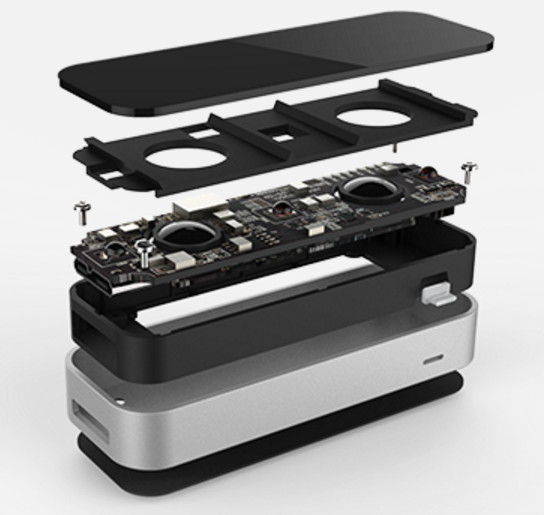
\includegraphics[width=6cm]{Bilder/leap-motion.png}			
		\caption{Explosionszeichnung der Leap Motion.~\cite{website:LeapMotionBlog}}
		\label{fig:leapMotion}
\end{figure}

\subsubsection{Leap Motion SDK} \label{sec:LeapSDK}\todo[inline, color=green] {Paul}
\textit{Leap Motion Inc.} bietet ein vollständiges Software Development Kit (SDK) für die \textit{Leap} an, welches \textit{Unity} um das Hand- und Fingertracking erweitert. Die Treibersoftware interpretiert die von den Kameras gelieferten Daten und sendet Trackinginformationen an die jeweilige Software. Das Leap SDK setzt an dieser Stelle an und verwendet diese eingehenden Daten um sie auf ein Handmodell in \textit{Unity} zu übertragen. Das SDK ist so vorbereitet, dass der Nutzer fertige Bausteine in die virtuelle Szene einbinden kann, die sich dann um die Dateninterpretation und visualisierung als Handmodelle kümmert. Die Handmodelle, die das SDK liefert, sind mit Collidern ausgestattet. Diese abstrahierte Geometrie lässt \textit{Unity} Kollisionen feststellen. Dieses Feature wird bei \textit{MArC} verwendet, um die Interaktion mit den virtuellen Menüelementen zu realisieren.\\
\textit{Leap} bietet zudem mehrere sog. "Module" an, die das SDK erweitern können. Unter anderem auch ein Modul, welches die \textit{Unity}-internen GUI Elemente mit den Handmodellen bedienbar machen. Nach einigen Tests hat sich jedoch herausgestellt, dass diese Interaktionsmöglichkeit für \textit{MArC} ungeeignet ist, da sie zu instabil läuft. Das um das UI Modul erweiterte SDK projiziert die Position der Fingerspitzen auf die UI Ebene, falls sich die Hand in der Nähe dieser befindet. Auf der UI wird dann ein kleiner Kreis angezeigt, um dem Nutzer ein visuelles Feedback zu gewährleisten.\\
Im Falle von \textit{MArC} sollten die virtuellen UI Elemente auf den Tisch platziert werden. Hierbei sind die Elemente jedoch immer ein wenig oberhalb des Tisches platziert, damit sie in jedem Fall mit der virtuellen Hand bedient werden können. Zwingend durchdringt die Hand dann die UI Elemente. Mittels des mitgelieferten UI-Modules ist eine Interaktion dann nicht mehr möglich. Daher war eine Bedienung mit Hilfe der Collider sinnvoller.

\subsubsection{ArUco Marker} \label{sec:aruco} \todo[inline, color=green]{Vera}
Die ArUco Bibliothek ist ein Marker Tracking Modul von \textit{OpenCV} (siehe Kapitel \ref{sec:OpenCV}) kann für Augmented Reality (AR) Anwendungen genutzt werden und stellt für diese Anwendungen alle notwendigen Funktionalitäten zum Orten und Verifizieren der Codes sowie der anschließenden Pose Estimation der ermittelten Positionen zur Verfügung \cite{article:Aruco2014}. 
Die Marker bestehen ähnlich wie QR-Codes aus einer zweidimensionalen Matrix, mit schwarzen oder weißen Feldern, welche die kodierten Daten binär, wie in Abbildung \ref{fig:AllUsedArucoMarker}, darstellen.  Weiterführend kann die Anzahl der Bits variabel gewählt werden (siehe Abbildung \ref{fig:SizesArucoMarker}), je nachdem wie groß die gefragte Markeranzahl ist oder deren erforderliche Erkennbarkeit in sehr großen Entfernungen sowie kleinen Bildern. Um diese Vielzahl an verschiedenen Größen und IDs händeln zu können wurden sogenannte Dictionarys eingeführt \cite{article:ArucoDictGarridoJurado2015}. Diese Dictionarys bestehen aus Markern mit gleicher Bit-Anzahl und sind zusätzlich auf eine maximalen Anzahl von IDs begrenzt um ein möglichst hohe Performanz zu gewährleisten.\\


\begin{figure}[H] 
	\center 
	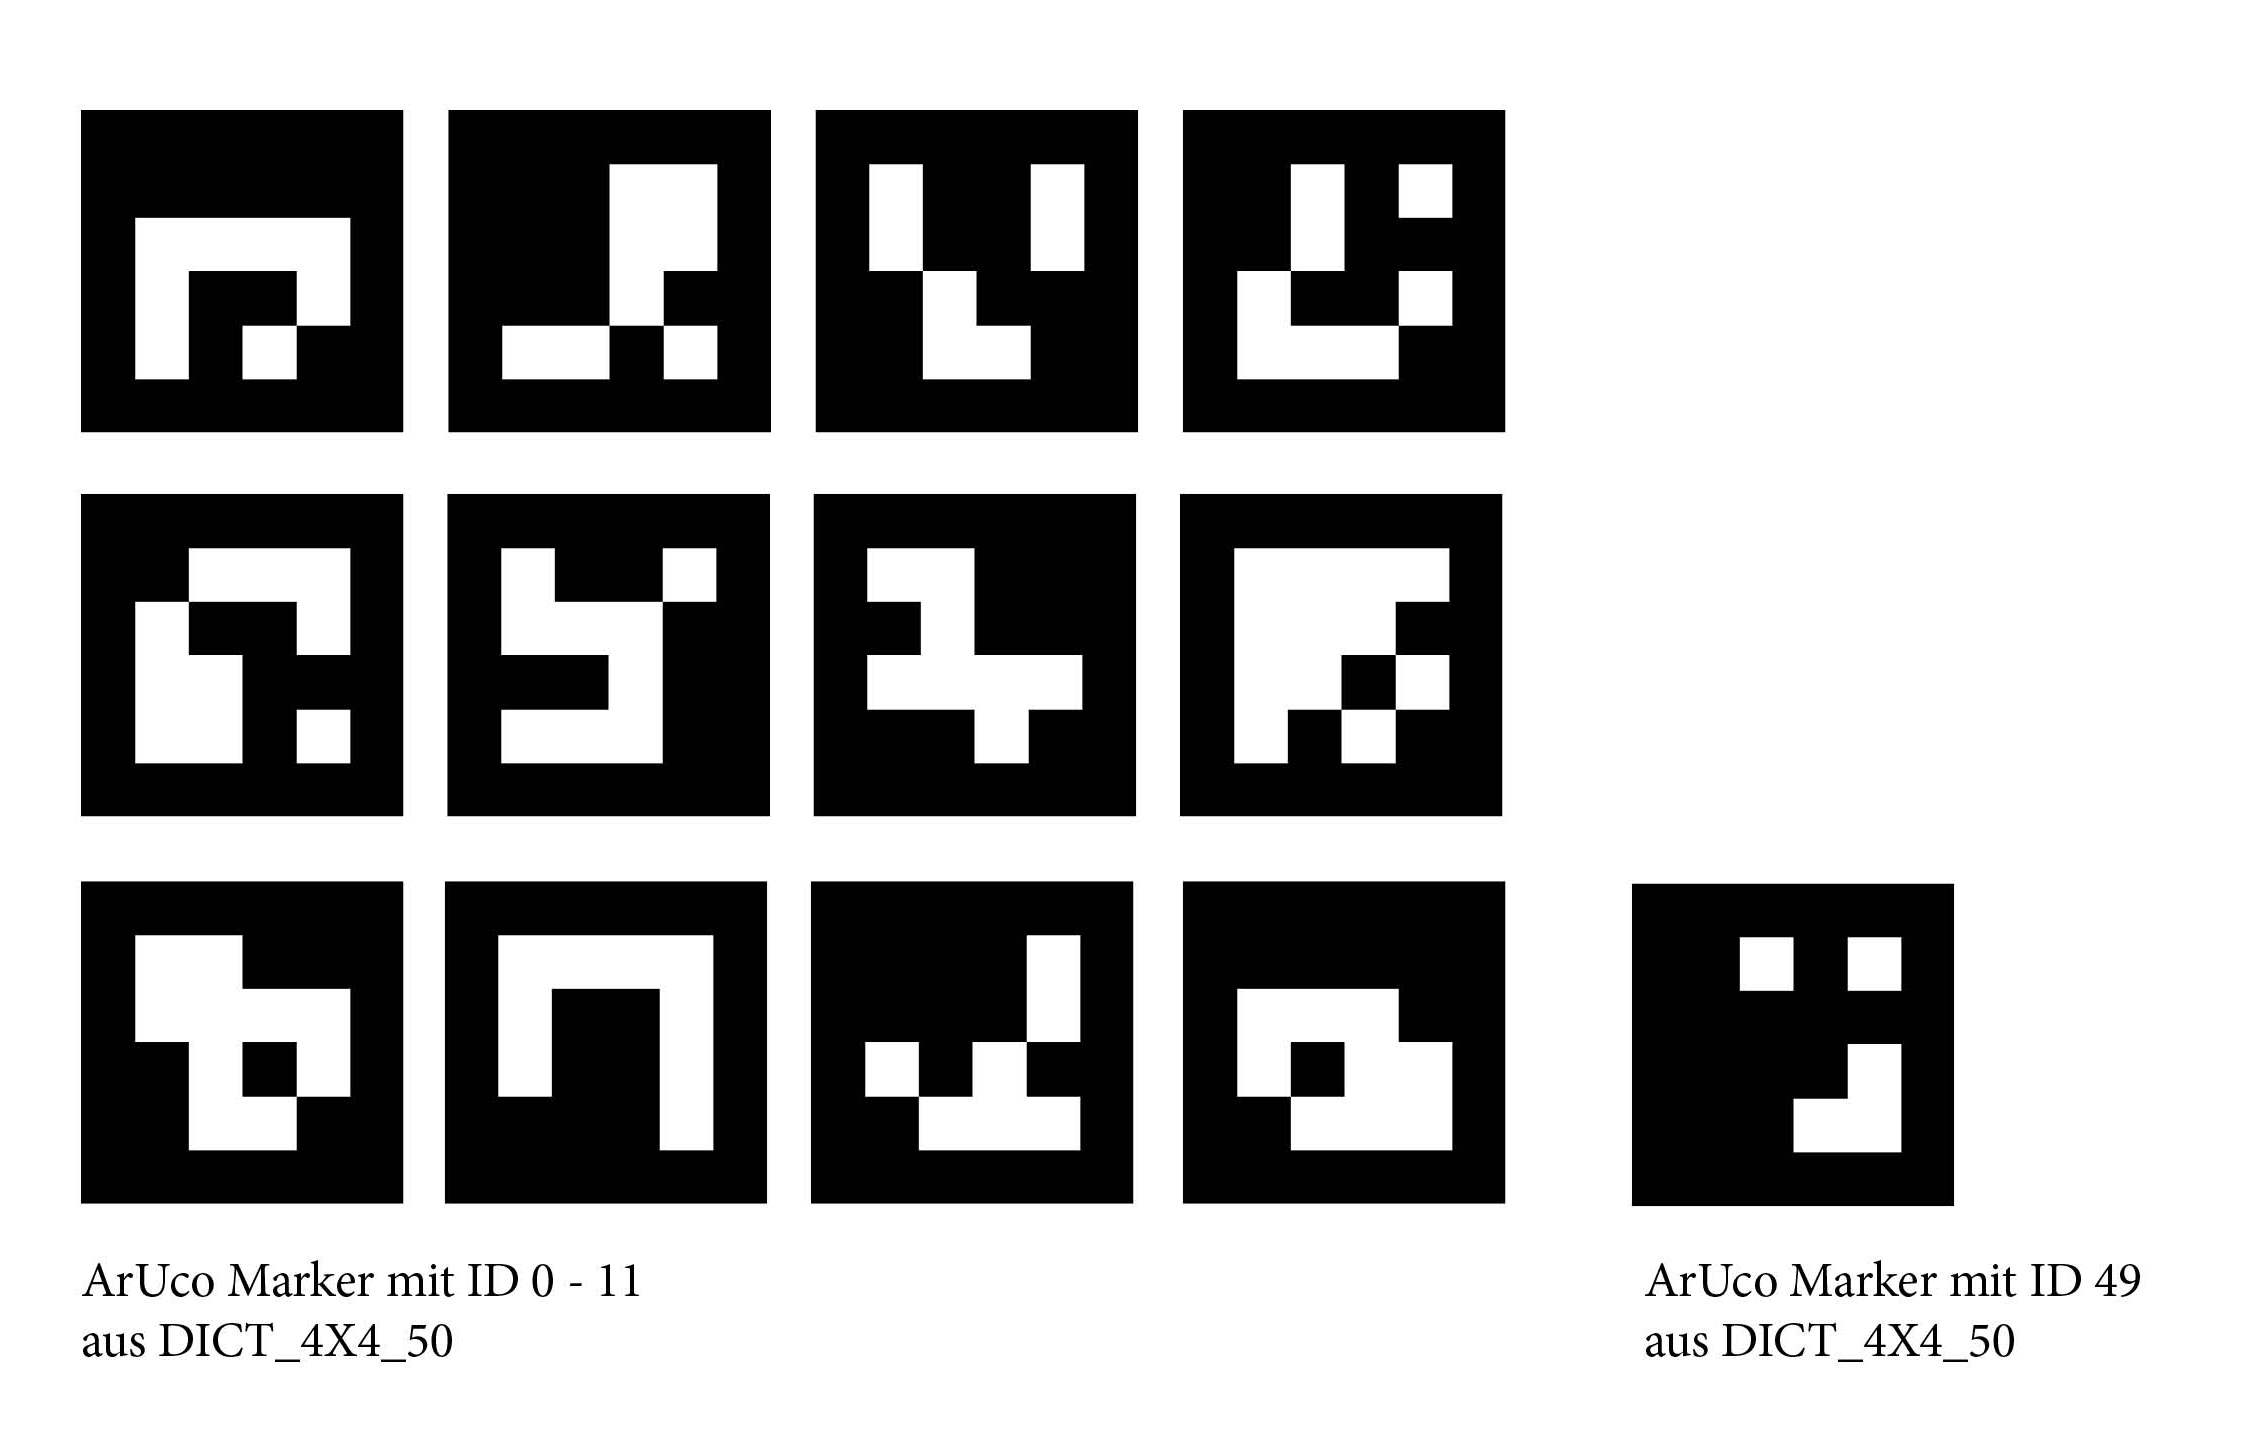
\includegraphics[width=10cm]{Bilder/Aruco_marker.jpg}			
	\caption{Alle genutzten 16 bit ArUco Marker des Prototypen. Links die zwölf IDs der Würfel Marker und rechts die ID, welche zur Kalibrierung benötigt wird. Die maximale Anzahl der Marker ist auf $50$ begrenzt.}
	\label{fig:AllUsedArucoMarker}
\end{figure}

\begin{figure}[H] 
	\center 
	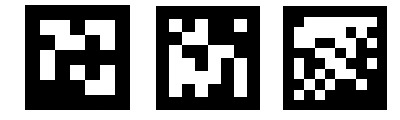
\includegraphics[width=7cm]{Bilder/VerschAruco.jpg}			
	\caption{ArUco Marker mit unterschiedlicher Bitgröße. Von Links nach Rechts: $n=5$, $n=6$ und $n=8$. Quelle: \cite{article:Aruco2014}}
	\label{fig:SizesArucoMarker}
\end{figure}

\subsubsection{Würfel Marker}\label{sec:WürfelMarker} \todo[inline, color=green]{Vera}

In vielen VR oder AR Umgebungen müssen die Nutzer eines Systems häufig nach virtuellen Objekten zur Interaktion greifen, die nicht real existieren. Demzufolge greifen die Personen ins Leere, was häufig die Immersion stört und zu Irritationen und Unsicherheit führt.
Um dem Nutzer des Systems \textit{MArC} für die Positionierung und Orientierung ein reales haptisches Feedback zu ermöglichen wurden zwölf Aluminumwürfel mit aufgeklebten Markern designt. Diese Würfel können beliebig innerhalb eines zuvor festgelegten Bereiches auf dem realen Tisch verschoben und rotiert werden. An der aktuellen Position und Orientierung des jeweiligen Markers wird in der VR ein explizit zugeordnetes Objekt gerendert. Diese Position wird mit Hilfe des Tracking-Algorithmus (siehe Kapitel \ref{sec:Tracking}) aus den Bildern der uEye Kamera ermittelt.
Alle zwölf Marker stimmen mit der Form und Farbe, sowie Material und Oberflächenbeschaffenheit aus Abbildung \ref{fig:marker} überein. Sie haben eine Kantenlänge von $46\,mm$ und sind in einem Winkel von $45^\circ$ an allen Kanten gefräst. Das Aluminium ist glasperlgestrahlt um eine matte Oberfläche zu erzeugen, welche ungewollte Reflexionen und Überstrahlungen vermeidet, die unter Umständen den Tracking-Algorithmus beeinflussen können. 

Auf die Oberseite des Markers ist mittig ein leuchtend grünes Quadrat mit einer Kantenlänge von $40\,mm$ aufgebracht. Diese grüne Fläche wird für ein Green-Keying benötigt, welches die Verfolgung der Marker auch bei Bewegungsunschärfe ermöglicht. Die leuchtend grüne Farbe wurde ausgewählt, da sie auf Grund ihrer hohen Leuchtkraft selten in der Natur und vor allem nicht in der Hautfarbe vorkommt. So hebt sie sich stark von ihrer Umgebung ab und erleichtert das Segmentieren der grünen Fläche im Bild. Die rechteckige Form der grünen Flächen hat noch eine weitere Bedeutung. Auf Grund der Geometrie können die äußeren Eckpunkt wie bei den rechteckigen codebasierten Markern auch zur Berechnung der Orientierung des Würfelmarkers im Kameraraum verwendet werden.

Ebenfalls mittig ist jeweils ein individueller $35\,mm$ großer $16$ bit ArUco-Marker plan befestigt. Alle verwendeten ArUco-Marker haben einen Rand von einem Bit hat und wurden jeweils aus dem Marker Dictionary $\texttt{DICT\_4X4\_50}$ des Arcuo Moduls \cite{website:ArucoDoc} generiert. Die maximale Anzahl an IDs von $50$ ist ausreichend für den Prototypen von \textit{MArC}, da die Anzahl von $50$ Würfelmarkern die durchschnittliche Fläche mehr als ausfüllen würde. Ein weiterer Vorteil dieser verhältnismäßig kleinen Dictonarys ist, dass auch der Aufwand für den entsprechenden Abgleich einer ID mit den potentiellen Mustern im Dictonary erheblich reduziert werden kann. 
Weiterführend beinhaltet das $\texttt{DICT\_4X4\_50}$ Dictionary auf Grund seiner $16$ bit Codierung sehr grobe und einfache Muster, welche gegen die mögliche Bewegungsunschärfe robuster ist. Bei sehr feinen Strukturen kann es schneller zu einer Verwischung des gesamten Musters kommen und die Wahrscheinlichkeit einer erfolgreichen Erkennung sinkt.
	\begin{figure}[H] 
	\center 
	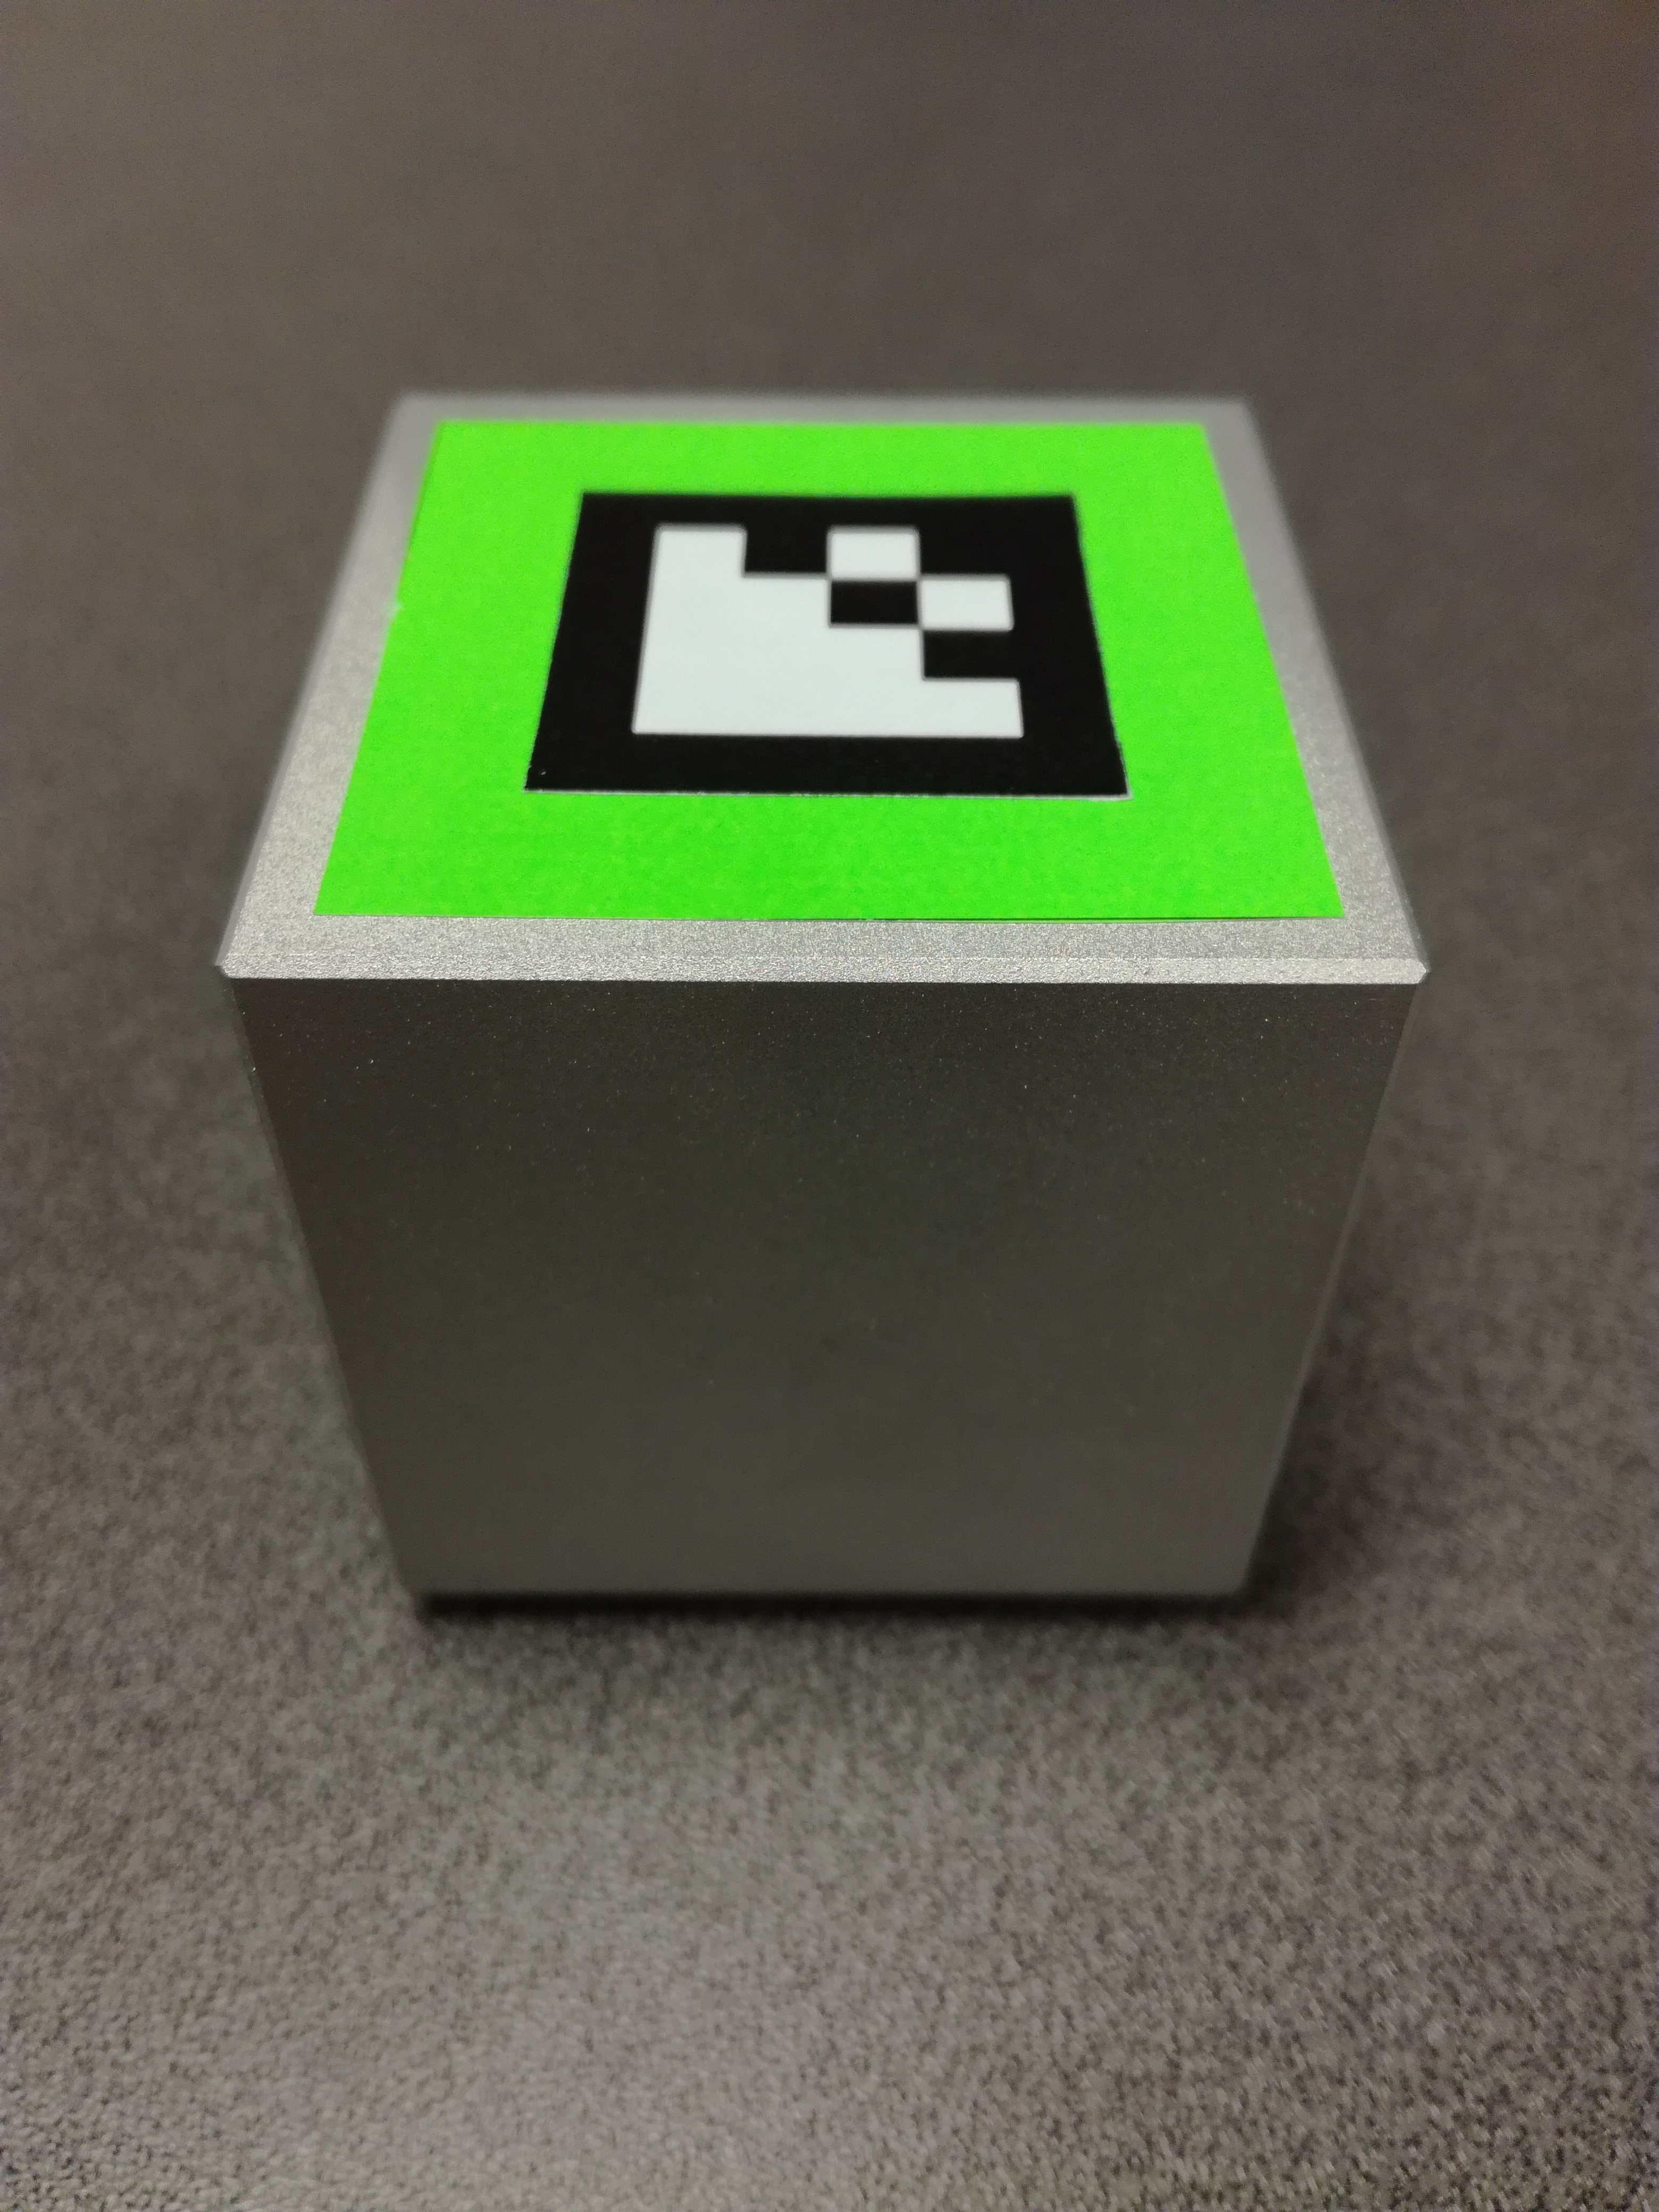
\includegraphics[trim = 0mm 280mm 0mm 150mm, clip, width=6cm]{Bilder/tracking-marker.jpg}			
	\caption{Würfel Marker mit grüner Fläche und einem ArUco Marker, die mittig auf den Aluminumwürfel aufgebracht sind.}
	\label{fig:marker}
\end{figure}

\subsubsection{Schachbrett-Kalibrierungshelfer zur Kamerakalibrierung} \label{sec:SchachbrettKalib} \todo[inline, color=yellow]{Laura}
Der in Abbildung~\ref{fig:schachbrettKalib} gezeigte Kalibrierungshelfer wird für die Kamerakalibrierung (vgl. Kapitel~\ref{sec:camCalib} der uEye-Kamera, deren Eigenschaften in Kapitel \ref{sec:uEye} beschrieben werden, verwendet. Dazu wurde eine Tisch-artige Erhöhung gebaut, die genauso hoch ist, wie die Würfel Marker (vgl. Kapitel \ref{sec:WürfelMarker}). Darauf ist ein ausgedrucktes Schachbrettmuster mit $6\times8$ Feldern, welches \textcolor{red}{VEEEEEERAAAAA: wo hatten wir das noch mal her?} zu finden ist.

	\begin{figure}[H] 
	\center 
	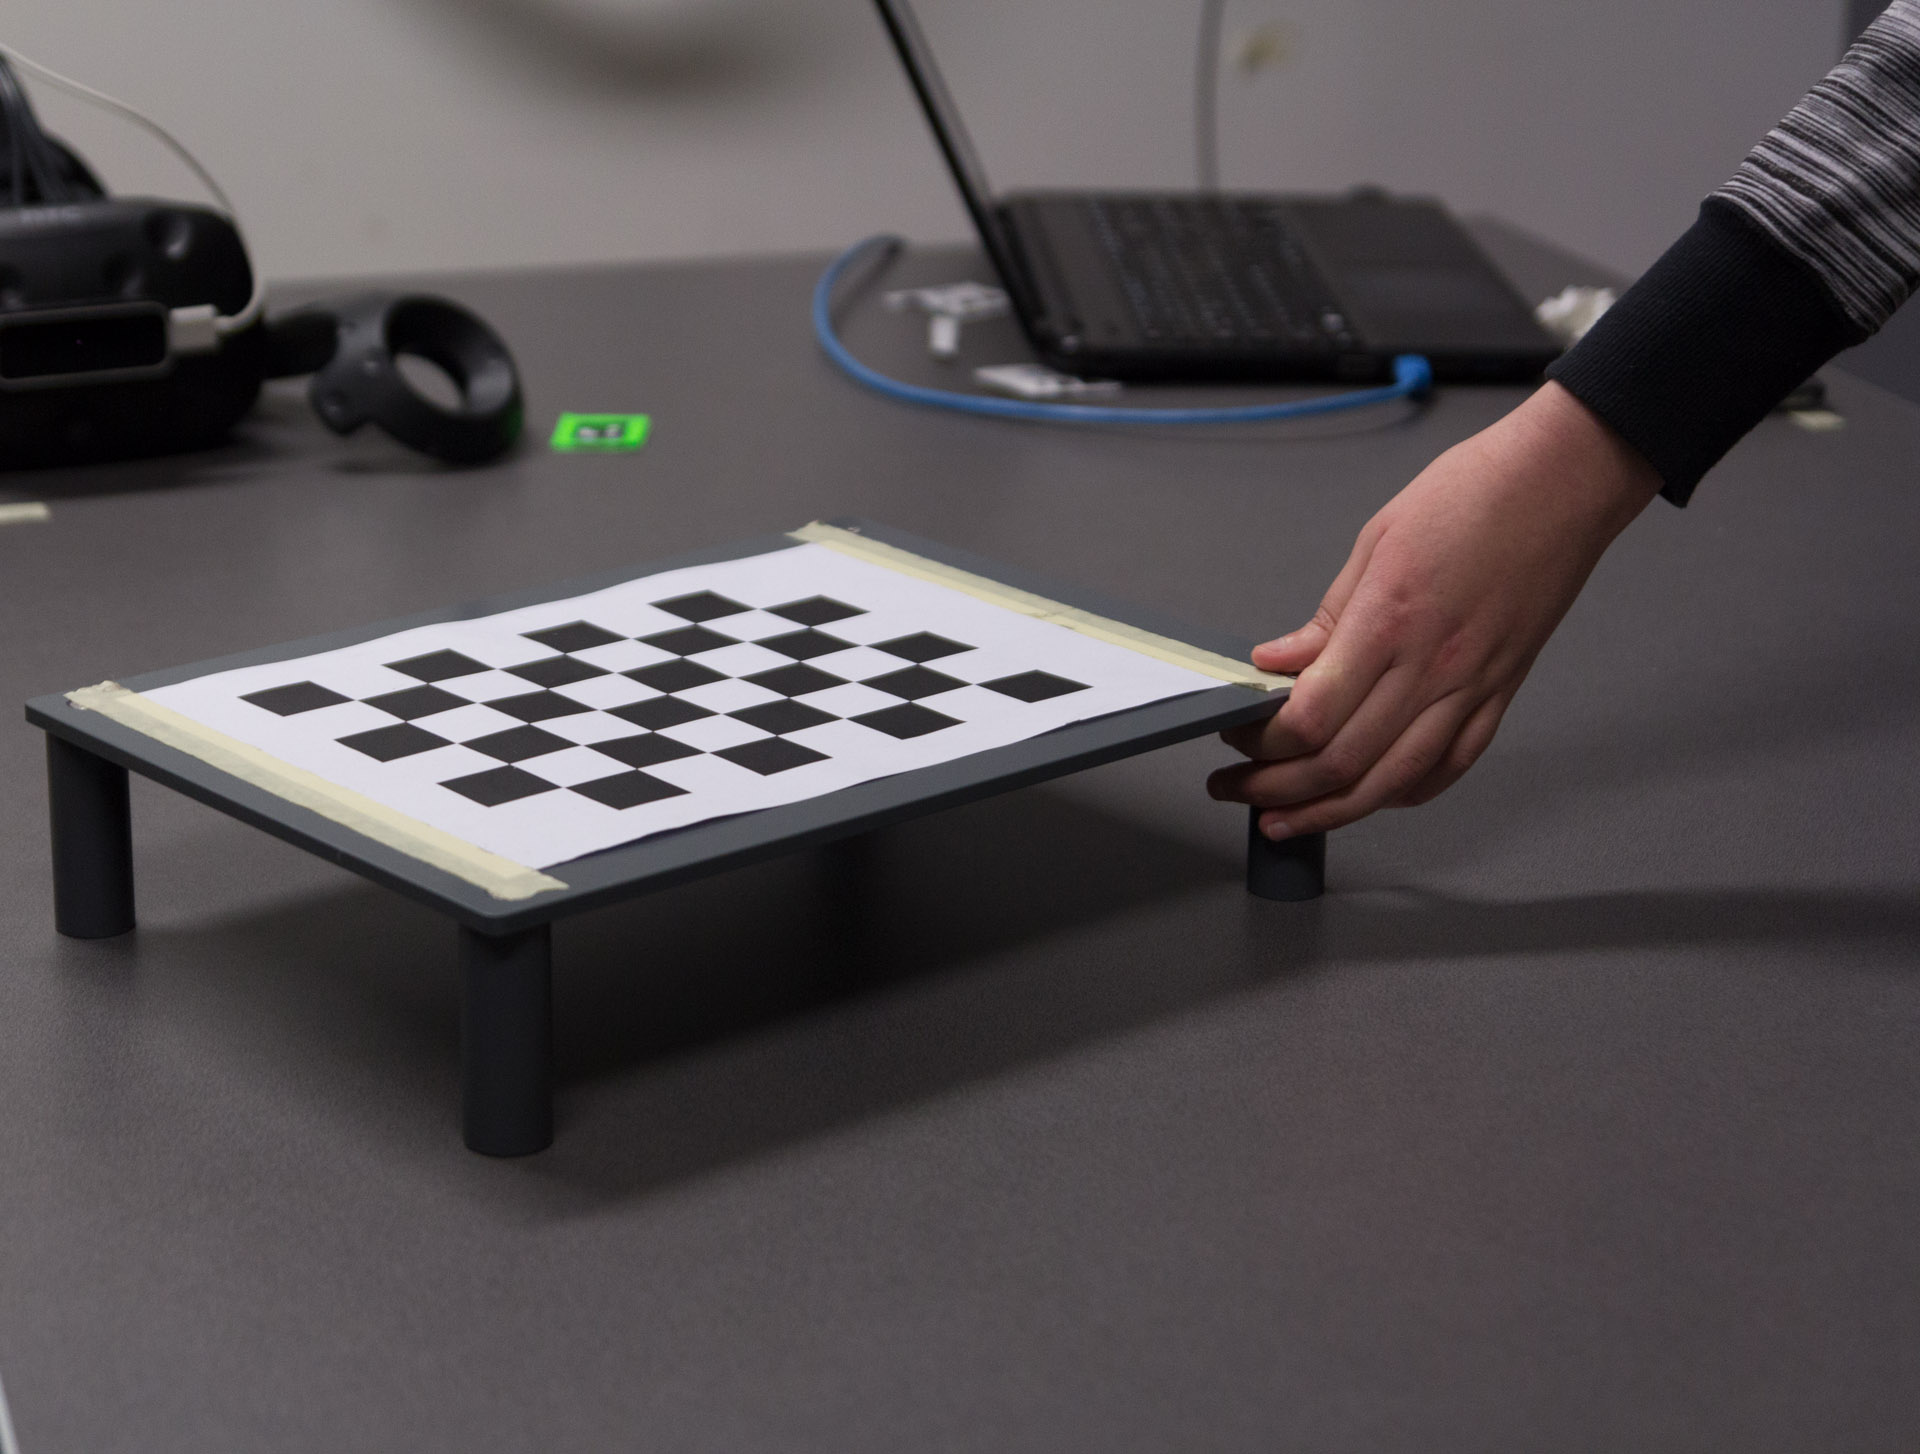
\includegraphics[trim = 0mm 20mm 30mm 30mm, clip]{Bilder/Eigene Fotos/IMG_0004.jpg}			
	\caption{Schachbrett-Kalibrierungshelfer.}
	\label{fig:schachbrettKalib}
\end{figure}

	
\subsection{Obsolete Hardware}\label{sec:obsoleteHardware}\todo[inline, color=green] {Lukas}
Im Laufe eines Projekts nach Art von \emph{MArC} ist es kaum vermeidbar, dass die gesetzten Projektziele reevaluiert werden müssen. Die Gründe hierfür können vielfältig sein. Beispielsweise könnte die Fertigstellung eines bestimmten Teils des Projekts deutlich länger gedauert haben als geplant, oder es könnte sich herausgestellt haben, dass bestimmte Komponenten zueinander nicht kompatibel sind.

Im vorliegenden Projekt trat eine Kombination der beiden oben genannten Gründe auf. Das Betreiben der \emph{Ovrvision Pro} Stereokamera, welche in Abschnitt~\ref{sec:ovrvision} kurz vorgestellt wird, am US-Bus verschiedener während der Entwicklung verwendeter Computer stellte sich als unberechenbar und damit leider unbenutzbar heraus. Die Kamera sorgte während der Ausführung von Unity dafür, dass mit allen anderen Geräten, die ebenfalls per USB angeschlossen waren, unterschiedlichste Probleme auftraten. Als die Situation nach dem Verbinden der Kamera in der teilweisen Zerstörung eines Mainboards gipfelte, wurde die Entscheidung getroffen, die \emph{Ovrvision Pro} nicht länger als Gerät in der Entwicklung von \emph{MArC} zu verwenden.

Stattdessen reifte zu diesem Zeitpunkt die Idee, eine gewöhnliche Webcam zu verwenden, um die Realisierung von Augmented Reality dennoch zu ermöglichen, wenn auch ohne den Stereo-3D-Effekt, welchen die \emph{Ovrvision Pro} nativ bereitgestellt hätte.

Im weiteren Verlauf des Projekts führte eine, lange Zeit ungeklärte, starke Abweichung der Positionen der realen und virtuellen Marker zur Neuordnung der Projektprioritäten. Dies hatte zur Folge, dass letztendlich auch die Webcam als Plattform für die Umsetzung der AR-Fähigkeiten von \emph{MArC} aufgegeben wurde und stattdessen auf eine reine VR-Lösung der Projekt-Problemstellung umgeschwenkt wurde.

Nachfolgend werden die Eigenschaften und technischen Daten beider Geräte kurz beschrieben.
\subsubsection{Ovrvision Pro}\label{sec:ovrvision}\todo[inline, color=green]{Lukas}
Die \emph{Ovrvision Pro} (vgl. Abb.~\ref{fig:ovr}) ist eine kompakte Stereokamera, welche über USB 3.0 mit einem Computer verbunden wird.~\cite{website:ovrvision} Für die Kamera ist eine Vielzahl an Software-Development-Kits (SDKs) für verschiedene Plattformen und Frameworks, wie etwa Microsoft Windows, Linux, Apple Mac OS X, Unreal Engine oder Unity verfügbar.~\cite{website:ovrvisionSetup}

Die \emph{Ovrvision Pro} ist speziell auf Augmented Reality (AR) Anwendungen ausgelegt. So unterstützt die Kamera natives Stereo-3D und bietet auch Bildmodi mit hohen Bildwiederholraten, welche für die Verwendung mit VR-Hardware wie Oculus Rift oder HTC Vive notwendig sind, um die Immersion des Benutzers nicht durch zu träge Bewegungswiedergabe zu beeinflussen. Die unterstützten Bildmodi der Kamera sind in Tabelle~\ref{tab:ovrRes} aufgeführt. Wie aus Abschnitt~\ref{sec:Vive} hervorgeht, stellt die HTC Vive Bildinhalte mit $1080\times1200$\,Pixeln pro Auge bei $90$\,Hz Bildwiederholrate da. Diese Leistung wird von der \emph{Ovrvision Pro} nicht erreicht.

\begin{table}
	\centering
	\begin{tabular}{|c|c|c|c|}
		\hline
		\Absatzbox{}
		\textbf{Örtliche Auflösung}& \textbf{Zeitliche} & \multicolumn{2}{c|}{\textbf{Bildwinkel}}\\
		\cline{3-4}
		\Absatzbox{}
		\textbf{pro Auge}& \textbf{Auflösung} & \textbf{Horizontal} & \textbf{Vertikal}\\
		\hline
		$2560\times1920$\,px & $15$\,fps & $115^\circ$ & $105^\circ$\\
		\hline
		$1920\times1080$\,px & $30$\,fps & $87^\circ$ & $60^\circ$\\
		\hline
		$1280\times960$\,px & $45$\,fps & $115^\circ$ & $105^\circ$\\
		\hline
		$1280\times800$\,px & $60$\,fps & $115^\circ$ & $90^\circ$\\
		\hline
		$960\times950$\,px & $60$\,fps & $100^\circ$ & $98^\circ$\\
		\hline
		$640\times480$\,px & $90$\,fps & $115^\circ$ & $105^\circ$\\
		\hline
		$320\times240$\,px & $120$\,fps & $115^\circ$ & $105^\circ$\\
		\hline
	\end{tabular}
	\caption{Bildmodi der \emph{Ovrvision Pro} Stereokamera.~\cite{website:ovrvisionProduct}}
	\label{tab:ovrRes}
\end{table}


\begin{figure}[H]
	\centering
	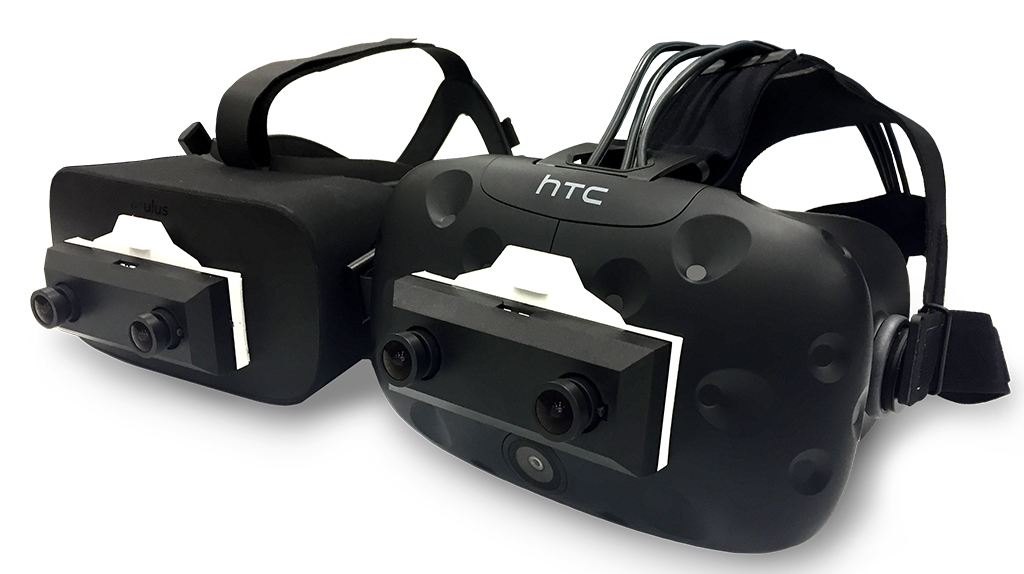
\includegraphics[width=\textwidth]{Bilder/ovr.jpg}			
		\caption{\emph{Ovrvision Pro} Stereokamera montiert an \emph{Oculus Rift} (links) und \emph{HTC Vive} (rechts).~\cite{website:ovrvision}}
		\label{fig:ovr}
\end{figure}
\subsubsection{Webcam}\label{sec:webcam} \todo[inline, color=green]{Vera}

Die \textit{Creative Senz3D} ist eine RGB Kamera mit einer zusätzlichen Infrarot-Tiefenkamera. Das generierte RGB-Bild hat eine Auflösung von $1280\times720$ Pixel und das Tiefenbild von $320\times240$ Pixel bei einer Reichweite von $15-99\,$cm sowie einem Sichtfeld von $74^\circ$. Die Kamera wird über eine USB 2.0 Schnittstelle mit einem Computer verbunden und nimmt Videos mit einer Framerate von bis zu $30$ fps auf \cite{website:Senz3d}. Weiter ist es möglich die Kamera direkt aus Anwendungen per \textit{Intel Perceptual Computing SDK} anzusteuern.

\subsection{Software} \todo[inline]{Vera}

Zur Entwicklung der \textit{MArC}-Software sind diverse Software-Komponenten und Bibliotheken notwendig. Die Funktionalitäten und Verwendung dieser Komponenten werden in diesem Kapitel kurz erläutert.


\subsubsection{Unity}\label{sec:unity}\todo[inline, color=green]{Lukas}

Unity ist eine sogenannte Spiel-Engine, also eine Entwicklungs- und Laufzeitumgebung, die speziell auf die Entwicklung von 3D-Spielen ausgelegt ist. Die Software wurde am 6. Juni 2005 veröffentlicht \cite{haas2014history} und wird von Unity Technologies \cite{website:Unity} entwickelt und vertrieben. In der Spieleentwicklung ist Unity weit verbreitet, so werden beispielsweise $34\,\%$ der kostenfreien Top-1000-Spiele im mobilen Sektor mit Unity entwickelt \cite{website:UnityPR}.

Unity bietet eine sehr breite Plattformunterstützung \cite{website:UnityMultiPlatform} und erlaubt ebenso die Entwicklung für Head-Mounted-Displays, wie etwa die Oculus Rift \cite{website:UnityOculus}\cite{website:UnityVRoverview} oder auch die in diesem Projekt verwendete HTC Vive \cite{website:UnityVRoverview}.

Die zu Beginn des Projekts verwendete Stereo-Kamera \emph{Ovrvision Pro} stellt ein Software-Development-Kit (SDK) für Unity (Version 5) zur Verfügung \cite{website:ovrvisionSetup}. Da das endgültige Resultat des Projekts die Verwendung der \emph{Ovrvision Pro} nicht mehr vorsieht, wie in~\ref{sec:obsoleteHardware} beschrieben, wird auf eine weitere Beschreibung dieses SDKs verzichtet.

\subsubsection{Visual Studio 2015}\label{sec:VisualStudio} \todo[inline, color=green] {Vera}

\textit{Micosoft Visual Studio 2015} ist eine verbreitete integrierte Entwicklungsumgebung (IDE), welche unter anderem die Programmiersprachen Visual Basic, Visual C$\#$, und Visual C++ unterstützt. Mit Hilfe dieser IDE kann ein Entwickler Win32/ Win64 Anwendungen sowie weitere WebApps und Webservices \cite{website:VisuStud} programmieren sowie anschließend compilieren. Für \textit{MArC} wurde mit der Version $14.0.25123.00$ Update2 gearbeitet.

\subsubsection{OpenCV} \label{sec:OpenCV} \todo[inline, color=green] {Vera}
\textit{Open Source Computer Vision} (OpenCV) ist eine Open Source Bibliothek für Bild- und Videoverarbeitung in der Programmiersprache \textit{C}$++$. Vorgestellt wurde sie vor über zehn Jahren von \textit{Intel} und wird seitdem stetig von verschiedenen Programmierern weiterentwickelt. Diese Bibliothek stellt die gängigsten Algorithmen sowie aktuelle Entwicklungen der Bildverarbeitung zur Verfügung
\cite{article:OpenCV}.\\
Für dieses System ist vor allem das Modul \texttt{calib3d} \cite{website:Calib3dDoc} und das extra Modul \texttt{aruco} \cite{website:ArucoDoc} verwendet. Das erste Modul \texttt{calib3d}  bietet alle notwendigen Funktionen zur Erstellung, Verwendung und Weiterverarbeitung von intrinsischen und extrinsischen Kamerakalibrierungen an (siehe Kapitel \ref{sec:calib}). Während das Zweite alle benötigten Ressourcen und Funktionalitäten zum Tracken von \textit{ArUco} Markern zur Verfügung stellt (siehe Kapitel \ref{sec:aruco}).

%\subsubsection{Orion Beta Software} \label{OBS}\todo[inline] {Paul}

\subsubsection{Steam VR}\todo[inline] {Paul}
\subsubsection{Windows Sockets (Winsock)}\label{sec:Winsock}\todo[inline, color=green] {Lukas}
Windows Sockets (abgekürzt Winsock) ist eine API für den Zugriff auf Netzwerkkomponenten in Microsoft Windows Betriebssystemen~\cite{quinn1998windows}. Winsock wird nativ in Microsoft Windows bereitgestellt.\\ 
Für die unkomplizierte Übertragung zwischen zwei Anwendungen in einem lokalen Netzwerk bieten sich sowohl das \emph{Transmission Control Protocol} (TCP), als auch das User \emph{User Datagram Protocol} (UDP) an. Das Erstellen von Netzwerk-Sockets für die Übertragung per TCP und UDP wird von Winsock ermöglicht.\\ Die Umsetzung der Netzwerkverbindung in \emph{MArC} wird in Abschnitt~\ref{sec:netzwerk} näher beschrieben.
\newpage